\documentclass[11pt,a4paper]{article}

% ----- preamble.tex -----
% % ----- preamble.tex -----
% % ----- preamble.tex -----
% \input{preamble.tex} should be included in all note files before '\begin{document}'
% \lecture{<lectureNumber>: <lectureTopic>}{<mm/dd/yyyy>}{<lecturerName>}{<authorName>}

\hbadness=10000
\vbadness=10000

% page size settings
\setlength{\textheight}{8.5in}
\setlength{\textwidth}{6.0in}
\setlength{\headheight}{0in}
\addtolength{\topmargin}{-.5in}
\addtolength{\oddsidemargin}{-.5in}

% paragraph spacing/indenting settings
\setlength\parindent{0pt}
\setlength\parskip{2.5pt}

% imported packages
\usepackage{amsmath,amssymb,amsthm}
\usepackage{mdframed} % for boxing
\usepackage{graphicx} % for inserting images
\graphicspath{ {./imgs/} }

\usepackage{diagbox} % backslash for tabular/tables
\usepackage{booktabs} % enhances quality of table presentation
\usepackage{tikz}
\usetikzlibrary{arrows,automata,trees,calc}

% ----- \tableofcontents PAGE LINKING (without blue highlight) -----
\usepackage{hyperref}
\hypersetup{
    colorlinks,
    citecolor=black,
    filecolor=black,
    linkcolor=black,
    urlcolor=black
}

% ----- VARIABLE RE-DEFINITIONS -----
\def\epsilon{\varepsilon}
\def\phi{\varphi}


% ----- TODO: MAKE EVERY NEW SECTION START ON NEW PAGE EXCLUDING TOC -----
% \let\oldsection\section
% \renewcommand{\section}{\newpage\oldsection}


% ----- CUSTOM COMMANDS -----
\newcommand{\handout}[5]{
    % \renewcommand{\thepage}{#1-\arabic{page}}
    \noindent
    \begin{center}
        \framebox{
            \vbox{
                \hbox to 5.78in {{\bf CS 4510: Automata and Complexity}\hfill #2}
                \vspace{4mm}
                \hbox to 5.78in {{\Large \hfill #5  \hfill}}
                \vspace{2mm}
                \hbox to 5.78in {{\it #3 \hfill #4}}
            }
        }
   \end{center}
   \vspace*{4mm}
}

\newcommand{\lecture}[4]{\handout{#1}{#2}{Lecturer: #3}{Author: #4}{Lecture #1}}

% keeps contents of the same theorem on the same page
\newcommand{\blocktheorem}[1]{
    \csletcs{old#1}{#1}
    \csletcs{endold#1}{end#1}
    \RenewDocumentEnvironment{#1}{o}{
        % \par\addvspace{cm}
        \noindent\begin{minipage}{\textwidth}
        \IfNoValueTF{##1}{\csuse{old#1}}{\csuse{old#1}[##1]}}{\csuse{endold#1}
        \end{minipage}
        \par\addvspace{0.75cm}
    }
}
\raggedbottom

\theoremstyle{definition}
\newtheorem{example}{Example} % use for example problems
\newmdtheoremenv{definition}{Definition} % use for definitions
\newtheorem{theorem}{Theorem} % use for theorems
\newtheorem{corollary}{Corollary} % use for corollary
\newtheorem{lemma}{Lemma} % use for corollary
\newtheorem{claim}{Claim}

\blocktheorem{example}
\blocktheorem{definition}
\blocktheorem{theorem}
\blocktheorem{corollary}
\blocktheorem{lemma}
\blocktheorem{claim} should be included in all note files before '\begin{document}'
% \lecture{<lectureNumber>: <lectureTopic>}{<mm/dd/yyyy>}{<lecturerName>}{<authorName>}

\hbadness=10000
\vbadness=10000

% page size settings
\setlength{\textheight}{8.5in}
\setlength{\textwidth}{6.0in}
\setlength{\headheight}{0in}
\addtolength{\topmargin}{-.5in}
\addtolength{\oddsidemargin}{-.5in}

% paragraph spacing/indenting settings
\setlength\parindent{0pt}
\setlength\parskip{2.5pt}

% imported packages
\usepackage{amsmath,amssymb,amsthm}
\usepackage{mdframed} % for boxing
\usepackage{graphicx} % for inserting images
\graphicspath{ {./imgs/} }

\usepackage{diagbox} % backslash for tabular/tables
\usepackage{booktabs} % enhances quality of table presentation
\usepackage{tikz}
\usetikzlibrary{arrows,automata,trees,calc}

% ----- \tableofcontents PAGE LINKING (without blue highlight) -----
\usepackage{hyperref}
\hypersetup{
    colorlinks,
    citecolor=black,
    filecolor=black,
    linkcolor=black,
    urlcolor=black
}

% ----- VARIABLE RE-DEFINITIONS -----
\def\epsilon{\varepsilon}
\def\phi{\varphi}


% ----- TODO: MAKE EVERY NEW SECTION START ON NEW PAGE EXCLUDING TOC -----
% \let\oldsection\section
% \renewcommand{\section}{\newpage\oldsection}


% ----- CUSTOM COMMANDS -----
\newcommand{\handout}[5]{
    % \renewcommand{\thepage}{#1-\arabic{page}}
    \noindent
    \begin{center}
        \framebox{
            \vbox{
                \hbox to 5.78in {{\bf CS 4510: Automata and Complexity}\hfill #2}
                \vspace{4mm}
                \hbox to 5.78in {{\Large \hfill #5  \hfill}}
                \vspace{2mm}
                \hbox to 5.78in {{\it #3 \hfill #4}}
            }
        }
   \end{center}
   \vspace*{4mm}
}

\newcommand{\lecture}[4]{\handout{#1}{#2}{Lecturer: #3}{Author: #4}{Lecture #1}}

% keeps contents of the same theorem on the same page
\newcommand{\blocktheorem}[1]{
    \csletcs{old#1}{#1}
    \csletcs{endold#1}{end#1}
    \RenewDocumentEnvironment{#1}{o}{
        % \par\addvspace{cm}
        \noindent\begin{minipage}{\textwidth}
        \IfNoValueTF{##1}{\csuse{old#1}}{\csuse{old#1}[##1]}}{\csuse{endold#1}
        \end{minipage}
        \par\addvspace{0.75cm}
    }
}
\raggedbottom

\theoremstyle{definition}
\newtheorem{example}{Example} % use for example problems
\newmdtheoremenv{definition}{Definition} % use for definitions
\newtheorem{theorem}{Theorem} % use for theorems
\newtheorem{corollary}{Corollary} % use for corollary
\newtheorem{lemma}{Lemma} % use for corollary
\newtheorem{claim}{Claim}

\blocktheorem{example}
\blocktheorem{definition}
\blocktheorem{theorem}
\blocktheorem{corollary}
\blocktheorem{lemma}
\blocktheorem{claim} should be included in all note files before '\begin{document}'
% \lecture{<lectureNumber>: <lectureTopic>}{<mm/dd/yyyy>}{<lecturerName>}{<authorName>}

\hbadness=10000
\vbadness=10000

% page size settings
\setlength{\textheight}{8.5in}
\setlength{\textwidth}{6.0in}
\setlength{\headheight}{0in}
\addtolength{\topmargin}{-.5in}
\addtolength{\oddsidemargin}{-.5in}

% paragraph spacing/indenting settings
\setlength\parindent{0pt}
\setlength\parskip{2.5pt}

% imported packages
\usepackage{amsmath,amssymb,amsthm}
\usepackage{mdframed} % for boxing
\usepackage{graphicx} % for inserting images
\graphicspath{ {./imgs/} }

\usepackage{diagbox} % backslash for tabular/tables
\usepackage{booktabs} % enhances quality of table presentation
\usepackage{tikz}
\usetikzlibrary{arrows,automata,trees,calc}

% ----- \tableofcontents PAGE LINKING (without blue highlight) -----
\usepackage{hyperref}
\hypersetup{
    colorlinks,
    citecolor=black,
    filecolor=black,
    linkcolor=black,
    urlcolor=black
}

% ----- VARIABLE RE-DEFINITIONS -----
\def\epsilon{\varepsilon}
\def\phi{\varphi}


% ----- TODO: MAKE EVERY NEW SECTION START ON NEW PAGE EXCLUDING TOC -----
% \let\oldsection\section
% \renewcommand{\section}{\newpage\oldsection}


% ----- CUSTOM COMMANDS -----
\newcommand{\handout}[5]{
    % \renewcommand{\thepage}{#1-\arabic{page}}
    \noindent
    \begin{center}
        \framebox{
            \vbox{
                \hbox to 5.78in {{\bf CS 4510: Automata and Complexity}\hfill #2}
                \vspace{4mm}
                \hbox to 5.78in {{\Large \hfill #5  \hfill}}
                \vspace{2mm}
                \hbox to 5.78in {{\it #3 \hfill #4}}
            }
        }
   \end{center}
   \vspace*{4mm}
}

\newcommand{\lecture}[4]{\handout{#1}{#2}{Lecturer: #3}{Author: #4}{Lecture #1}}

% keeps contents of the same theorem on the same page
\newcommand{\blocktheorem}[1]{
    \csletcs{old#1}{#1}
    \csletcs{endold#1}{end#1}
    \RenewDocumentEnvironment{#1}{o}{
        % \par\addvspace{cm}
        \noindent\begin{minipage}{\textwidth}
        \IfNoValueTF{##1}{\csuse{old#1}}{\csuse{old#1}[##1]}}{\csuse{endold#1}
        \end{minipage}
        \par\addvspace{0.75cm}
    }
}
\raggedbottom

\theoremstyle{definition}
\newtheorem{example}{Example} % use for example problems
\newmdtheoremenv{definition}{Definition} % use for definitions
\newtheorem{theorem}{Theorem} % use for theorems
\newtheorem{corollary}{Corollary} % use for corollary
\newtheorem{lemma}{Lemma} % use for corollary
\newtheorem{claim}{Claim}

\blocktheorem{example}
\blocktheorem{definition}
\blocktheorem{theorem}
\blocktheorem{corollary}
\blocktheorem{lemma}
\blocktheorem{claim}

\begin{document}
\lecture{5: NFA To DFA}{09/06/2022}{Zvi Galil}{Austin Peng}
\tableofcontents

% TODO: how do i fix this to have new page before every section, but not before the table of contents
\AddToHook{cmd/section/before}{\newpage}

\section{Equivalence Of NFAs and DFAs (cont.)}
\begin{theorem}
    Every NFA has an equivalent DFA.

    \begin{proof}
        Let $N=(Q,\Sigma,\delta,q_0, F)$ be the NFA recognizing some language $A$. We construct DFA $M=(Q',\Sigma,\delta',q'_0,F')$ recognizing $A$.
        Before doing the full construction, first consider the easier case when $N$ has no $\epsilon$ arrows. We will take $\epsilon$ into account later.

        \begin{enumerate}
            \item $Q'=\mathcal{P}(Q)$ (the set of subsets of $Q$)
            \subitem Every state of $M$ is a set of states of $N$.
            \item $\Sigma$ (the alphabet) doesn't change
            \item For $R\in Q'$, and $a\in\Sigma$, let $\delta'(R,a)=\{q\in Q\mid q\in\delta(r,a)\text{ for some }r\in R\}$
            \subitem If $R$ is a state of $M$, it is also a set of states of $N$. When $M$ reads a symbol $a$ in state $R$, it shows where $A$ takes each state in $R$. Because each state may go to a set of states, we take the union of all these sets.
            $$\delta'(R,a)=\bigcup\limits_{r\in R}\delta(r,a)$$
            \item $q'_0=\{q_0\}$
            \subitem $M$ starts in the state corresponding to the collection containing just the start state of $N$.
            \item $F'=\{R\in Q'\mid R\text{ contains an accepting state of }N\}$
            \subitem The machine $M$ accepts if one of the possible states that $N$ could be in at this point is an accepting state.
        \end{enumerate}

        Now consider the $\epsilon$ arrows. For any state $R$ of $M$, we define $E(R)$ to be the collection of states that can be reached from members of $R$ by going only along $\epsilon$ arrows, including members of $R$ themselves.
        Formally, for $R\subseteq Q$, let $$E(R)=\{q\mid q\text{ can be reached from $R$ by traveling along 0 or more $\epsilon$ arrows}\}$$
        Then we modify the transition function of $M$ to place additional fingers on all states that can be reached by going along $\epsilon$ arrows after every step. Replacing $\delta(r,a)$ by $E(\delta(r,a))$ achieves this.
        Finally, we need to modify the start state of $M$ to move the fingers initially to all possible states that can be reached from the start state of $N$ along the $\epsilon$ arrows. \\
        
        The changes mentioned above to account for $\epsilon$ arrows are shown below:
        \begin{enumerate}
            \setcounter{enumi}{2}
            \item $\delta'(R,a)=\{q\in Q\mid q\in E(\delta(r,a))\text{ for some }r\in R\}$
            \item $q'_0=E(\{q_0\})$
        \end{enumerate}
    \end{proof}
\end{theorem}

\begin{example}
    Consider the following NFA $N$:

    \begin{tikzpicture}[node distance={2.5cm}, semithick, main/.style = {draw, circle}]
        \node[name=input] {};
        \node[state,accepting] (0) [right of=input] {$1$};
        \node[state] (1) [below of=0] {$2$};
        \node[state] (2) [right of=1] {$3$};

        % q_0
        \draw[->] (input) -- (0);
        \draw[->] (0) to node[left] {$b$} (1);
        \draw[->,out=295,in=155] (0) to node[above] {$\epsilon$} (2);

        % q_1
        \path (1) edge [loop left] node {$a$} (1);

        % q_2
        \draw[->,out=115,in=335] (2) to node[left] {0} (0);
        \draw[->] (1) to node[below] {$a,b$} (2);
    \end{tikzpicture}

    Note that the DFA will have 8 states, one for each subset of the states of $N$. The DFA and its transitions are shown below: \\

    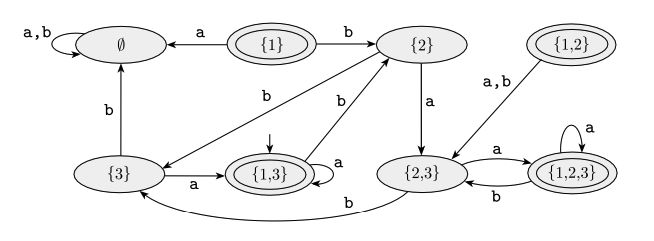
\includegraphics[width=\linewidth]{lecture05-dfa-equiv-of-nfa.png}

    The NFA's start state is $1$, so the DFA's start state is $E(\{1\})=\{1,3\}$ (the set of states reachable from $1$ by travelling along $\epsilon$ arrows and $1$ itself).
    The NFA's accepting state is $1$, so the DFA's accepting states are all sets of states that include $1$: $\{\{1\}, \{1,2\},\{1,3\},\{1,2,3\}\}$ \\

    As for $D$'s transition function, each of $D$'s states goes to one place on input $a$ and one place on input $b$ (by definition of DFA). We will illustrate a few.

    \begin{itemize}
        \item in $D$, state $\{2\}$ goes to $\{2,3\}$ on input $a$ because in $N$, state $2$ goes to both $2$ and $3$ on input $a$.
        \item in $D$, state $\{1\}$ goes to $\emptyset$ on input $a$ because no $a$ arrows exit it.
        \item in $D$, state $\{1,2\}$ goes to $\{2,3\}$ on input $a$ because in $N$, state $1$ goes nowhere on input $a$ and state $2$ goes to both $2$ and $3$ on input $a$
    \end{itemize}

    NFA with $n$ states $\rightarrow$ DFA with $2^n$ states.
\end{example}

\section{Closure Under Regular Operations}
\begin{theorem}
    The class of regular languages is closed under the union operation. \\

    \textit{Proof Idea.} We have regular languages $A_1$ and $A_2$ and want to prove that $A_1\cup A_2$ is regular.
    The idea is to take 2 NFAs, $N_1$ and $N_2$, that accept $A_1$ and $A_2$ respectively, and combine them into a single new NFA $N$.

    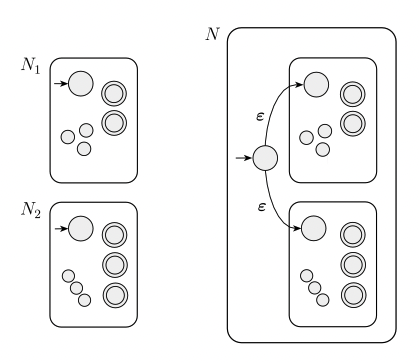
\includegraphics[width=\linewidth / 2]{lecture05-union-closure-nfa-proof-idea.png}
    \begin{proof}
        Let $N_1=(Q_1,\Sigma,\delta_1,q_1,F_1)$ recognize $A_1$ and $N_2=(Q_2,\Sigma,\delta_2,q_2,F_2)$ recognize $A_2$. \\

        Construct $N=(Q,\Sigma,\delta,q_0,F)$ to recognize $A_1\cup A_2$.

        \begin{enumerate}
            \item $Q=\{q_0\}\cup Q_1\cup Q_2$
            \subitem The states of $N$ are all the states of $N_1$ and $N_2$ with the addition of a new start state $q_0$.
            \item The state $q_0$ is the start state of $N$.
            \item The set of accepting states $F=F_1\cup F_2$.
            \subitem The accepting states of $N$ are all the accepting states of $N_1$ and $N_2$. That way, $N$ accepts if either $N_1$ or $N_2$ accepts.
            \item Define $\delta$ so that for any $q\in Q$ and any $a\in\Sigma_{\epsilon}$,
            $$\delta(q,a)=\begin{cases}
                \delta_1(q,a) & q\in Q_1 \\
                \delta_2(q,a) & q\in Q_2 \\
                \{q_1,q_2\} & q=q_0\text{ and }a=\epsilon \\
                \emptyset & q=q_0\text{ and }a\neq\epsilon
            \end{cases}$$
        \end{enumerate}
    \end{proof}
\end{theorem}

\begin{theorem}
    The class of regular languages is closed under the concatenation operation. \\

    \textit{Proof Idea.} We have regular languages $A_1$ and $A_2$ and want to prove that $A_1\circ A_2$ is regular.
    The idea is to take 2 NFAs, $N_1$ and $N_2$, and combine them into a single new NFA $N$ (like how we did in the union closure proof, but with a few changes).

    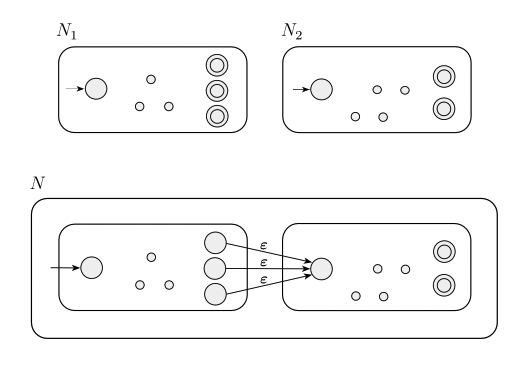
\includegraphics[width=\linewidth / 2]{lecture05-concat-closure-nfa-proof.png}

    \begin{proof}
        Let $N_1=(Q_1,\Sigma,\delta_1,q_1,F_1)$ recognize $A_1$ and $N_2=(Q_2,\Sigma,\delta_2,q_2,F_2)$ recognize $A_2$. \\

        Construct $N=(Q,\Sigma,\delta,q_0,F)$ to recognize $A_1\circ A_2$.

        \begin{enumerate}
            \item $Q=Q_1\cup Q_2$
            \subitem The states of $N$ are all the states of $N_1$ and $N_2$.
            \item The state $q_1$ is the start state of $N_1$.
            \item The set of accepting states $F_2$ are the same as the accepting states of $N_2$.
            \item Define $\delta$ so that for any $q\in Q$ and any $a\in\Sigma_{\epsilon}$,
            $$\delta(q,a)=\begin{cases}
                \delta_1(q,a) & q\in Q_1\text{ and }q\notin F_1 \\
                \delta_1(q,a) & q\in F_1\text{ and }a\neq\epsilon \\
                \delta_1(q,a)\cup\{q_2\} & q\in F_1\text{ and }a\in\epsilon \\
                \delta_2(q,a) & q\in Q_2
            \end{cases}$$
        \end{enumerate}
    \end{proof}
\end{theorem}

\begin{theorem}
    The class of regular languages is closed under the Kleene star operation. \\

    \textit{Proof Idea.} We have a regular language $A$ and want to prove that $A_1^*$ also is regular. We take an NFA $N_1$ for $A_1$ and modify it to recognize $A_1^*$ as shown.
    The resulting NFA $N$ will accept its input whenever it can be broken into several pieces and $N$ accepts each piece. \\

    We can construct $N$ like $N_1$ with additional $\epsilon$ arrows returning to the start state from the accepting states.
    This way when the processing gets to the end of a piece that $N_1$ accepts, the machine $N$ has the option of jumping back to the start state to try to read another piece that $N_1$ accepts.

    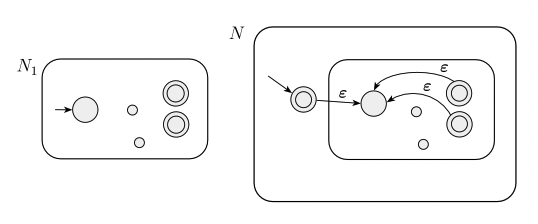
\includegraphics[width=\linewidth * 2 / 3]{lecture05-star-closure-nfa-proof.png}

    \begin{proof}
        Let $N_1=(Q_1,\Sigma,\delta_1,q_1,F_1)$ recognize $A_1$. Construct $N=(Q,\Sigma,\delta,q_0,F)$ to recognize $A_1^*$.

        \begin{enumerate}
            \item $Q=\{q_0\}\cup Q_1$
            \subitem The states of $N$ are the states of $N_1$ plus a new start state.
            \item The state $q_0$ is the new start state.
            \item $F=\{q_0\}\cup F_1$
            \subitem The accepting states are the old accepting states plus the new start state.
            \item Define $\delta$ so that for any $q\in Q$ and any $a\in\Sigma_{\epsilon}$,
            $$\delta(q,a)=\begin{cases}
                \delta_1(q,a) & q\in Q_1\text{ and }q\notin F_1 \\
                \delta_1(q,a) & q\in F_1\text{ and }a\notin\epsilon \\
                \delta_1(q,a)\cup\{q_1\} & q\in F_1\text{ and }a\in\epsilon \\
                \{q_1\} & q=q_0\text{ and }a\in\epsilon \\
                \emptyset & q=q_0\text{ and }a\notin\epsilon
            \end{cases}
            $$
        \end{enumerate}
    \end{proof}
\end{theorem}

\end{document}